\chapterimage{blue14.jpeg} % Imagen de encabezado de capítulo
\chapterspaceabove{6.75cm} % Espacio en blanco desde la parte superior de la página hasta el título del capítulo en las páginas del capítulo
\chapterspacebelow{7.25cm} % Cantidad de espacio en blanco vertical desde el margen superior hasta el comienzo del texto en las páginas de los capítulos

%------------------------------------------------

\chapter{TÉCNICAS DE CONTEO}\label{chap:2}


En el emocionante mundo de las Matemáticas Discretas, existen herramientas y métodos que nos permiten abordar problemas complejos de manera estructurada y precisa. Uno de los aspectos más fascinantes de este campo es la aplicación de las técnicas de conteo, una habilidad esencial para contar y cuantificar conjuntos finitos de objetos. Estas técnicas nos brindan la capacidad de analizar y resolver problemas relacionados con la cantidad de formas en que ciertos eventos pueden ocurrir, sin necesidad de enumerar cada posibilidad individualmente.

El capítulo que exploraremos a continuación se sumerge en el intrigante mundo de las técnicas de conteo en Matemáticas Discretas. Aquí descubriremos cómo contar y calcular de manera eficiente, evitando la repetición de casos y garantizando que no pasemos por alto ninguna posibilidad. Desde contar permutaciones y combinaciones hasta abordar problemas de distribución y partición, estas técnicas no solo son fundamentales en matemáticas, sino que también tienen aplicaciones en áreas como la informática, la estadística y la teoría de la probabilidad.\\



Las técnicas de conteo son más que simples procedimientos matemáticos; son herramientas poderosas que nos ayudan a desentrañar la complejidad de problemas aparentemente intrincados. A través de las técnicas de conteo en Matemáticas Discretas, descubriremos cómo contar, calcular y abordar desafíos con una claridad renovada y una habilidad recién adquirida.


\section{Reglas de la suma y el producto}

\begin{tcolorbox}[
      theorem style=change break,
      enhanced,
      breakable,
      boxrule=0pt,
      frame hidden,
      borderline west={3pt}{0pt}{jblueleft},
      colback=jblueinner,
      coltitle=jblueleft,
      attach title to upper={\ },
      sharp corners,
      title={Regla de la suma:},
      fonttitle=\bfseries,
      fontupper=\normalsize
]
    Si una primera tarea puede realizarse de $m$ formas, mientras que una segunda tarea puede realizarse de $n$ formas, y no es posible realizar ambas tareas de manera simultánea, entonces, para llevar a cabo cualquiera de ellas pueden utilizarse cualquiera de $m + n$ formas.
\end{tcolorbox}

\begin{myexample}
    La biblioteca de una universidad tiene 40 libros de texto de sociología y 50 de antropología. Por la regla de la suma, un estudiante de esta universidad puede elegir entre $40 + 50 = 90$ libros de texto para aprender acerca de alguno de estos dos temas.
\end{myexample}

\newpage 

\begin{tcolorbox}[
      theorem style=change break,
      enhanced,
      breakable,
      boxrule=0pt,
      frame hidden,
      borderline west={3pt}{0pt}{jblueleft},
      colback=jblueinner,
      coltitle=jblueleft,
      attach title to upper={\ },
      sharp corners,
      title={Regla del producto:},
      fonttitle=\bfseries,
      fontupper=\normalsize
]
    Si un procedimiento se puede descomponer en las etapas primera y segunda, y si existen $m$ resultados posibles de la primera etapa y si, para cada uno de estos resultados, existen $n$ resultados posibles para la segunda etapa, entonces el procedimiento total se puede realizar, en el orden dado, de $mn$ formas.
\end{tcolorbox}

\begin{importante}{}{}
    A la regla del producto también se le conoce como el \textbf{principio de elección}.
\end{importante}

\begin{myexample}
    En una oficina se solicita una secretaria y un supervisor. Si hay 5 candidatos para el puesto de secretaria y 5 candidatos para el puesto de supervisor, entonces por el principio del producto es posible asignar la pareja de puestos vacantes de $(5)(5) = 25$ formas distintas.
\end{myexample}

\begin{obs}{}{}
    Si asignamos a cada secretaria y supervisor con una letra respectivamente, es decir,
    \begin{center}
        \begin{tabular}{lccccc}
            Secretaria & a & b & c & d & e \\
            Supervisor & f & g & h & i & j
        \end{tabular}
    \end{center}
    Podemos mostrar las posibilidades del ejemplo anterior con un diagrama de árbol como sigue:\\
    
    \Tree[.{Número de vacantes} [.a [.f ] [.g ] [.h ] [.i ] [.j ] ] [.b [.f ] [.g ] [.h ] [.i ] [.j ] ] [.c [.f ] [.g ] [.h ] [.i ] [.j ] ] [.d [.f ] [.g ] [.h ] [.i ] [.j ] ] [.e [.f ] [.g ] [.h ] [.i ] [.j ] ] ]
\end{obs}

\section{Permutaciones}

\begin{definicion}{}{}
    Sea $n \in \ZZ[+]$. Definimos el \textbf{factorial} de $n$, denotado por $n!$, como
    $$n! = (n)(n-1)(n-2) \cdots (3)(2)(1).$$
\end{definicion}

\begin{myexample}
    Usando la definición anterior, si $n = 4$, entonces
    \begin{align*}
        4! & = (4)(4-1)(4-2)(4-3) \\
        & = (4)(3)(2)(1) \\
        & = 24.
    \end{align*}
\end{myexample}

\newpage

\begin{importante}{}{}
    Las permutaciones de objetos se pueden definir como las \textbf{ordenaciones} de estos mismos.
\end{importante}

\begin{myexample}
    Se quieren ordenar 5 libros distintos en un estante:
    \begin{center}
        \begin{tikzpicture}
            \draw[jblueleft] (0,0) rectangle (1,3);
            \draw[jblueleft] (1,0) rectangle (2,2);
            \draw[jblueleft] (2,0) rectangle (3,1.5);
            \draw[jblueleft] (3,0) rectangle (4,2.5);
            \draw[jblueleft] (4,0) rectangle (5,3);

            \node[jblueleft] at (0.5,1.5) {a};
            \node[jblueleft] at (1.5,1) {b};
            \node[jblueleft] at (2.5,0.75) {c};
            \node[jblueleft] at (3.5,1.25) {d};
            \node[jblueleft] at (4.5,1.5) {e};
        \end{tikzpicture}
    \end{center}
    Algunas ordenaciones son
    \begin{center}
        \begin{tabular}{ccccc}
            a & b & c & d & e \\
            c & a & b & c & d \\
            d & e & a & b & c
        \end{tabular}
    \end{center}
    Notemos que al aplicar el principio del producto, obtenemos
    \begin{align*}
        5! & = (5)(4)(3)(2)(1) \\
        & = 120 \text{ ordenaciones diferentes.}
    \end{align*}
\end{myexample}

\begin{notation*}{}
    Denotaremos al número de permutaciones como
    $$P(n, \, n) = {}_nP_n = n!.$$
\end{notation*}

\begin{myexample}
    A partir de un grupo de 10 personas se van a seleccionar 5 de ellas para formarlas en una fila de 5 sillas para fotografiarlas. ¿Cuántas permutaciones (ordenaciones) diferentes se pueden hacer?\\
    \newline
    \textbf{\color{jblueleft}Solución:} Si asignamos a cada persona una letra, es decir
    \begin{center}
        \begin{tabular}{ccccccccccc}
            Personas & a & b & c & d & e & f & g & h & i & j
        \end{tabular}
    \end{center}
    obtenemos
    \begin{center}
        \begin{tabular}{cccccccccc}
            10 & & 9 & & 8 & & 7 & & 6 \\
            primera & & segunda & & tercera & & cuarta & & quinta \\
            posición & & posición & & posición & & posición & & posición
        \end{tabular}
    \end{center}
    es decir,
    \begin{align*}
        P(10, \, 5) & = (10)(9)(8)(7)(10-5+1) \\ 
        & = 30 \, 240 \text{ ordenaciones.}
    \end{align*}
    Si se utiliza la notación factorial:
    \begin{displaymath}
        P(10, \, 5) = \frac{(10)(9)(8)(7)(6)(5)(4)(3)(2)(1)}{(5)(4)(3)(2)(1)} = \frac{10!}{5!} = \frac{10!}{(10-5)!}.
    \end{displaymath}
\end{myexample}

\begin{obs}{}{}
    En general, podemos obtener el número de permutaciones de tamaño $r$ para $n$ objetos como:
    \begin{center}
        \begin{tabular}{cccccccccc}
            $n$ & & $n-1$ & & $n-2$ & & $\cdots$ & & $n-r+1$ \\
            primera & & segunda & & tercera & &  & & $r$-ésima \\
            posición & & posición & & posición & &  & & posición
        \end{tabular}
    \end{center}
    es decir,
    $$P(n, \, r) = (n)(n-1)(n-2) \cdots (n-r+1).$$
    Incluyendo la notación factorial, obtenemos:
    $$P(n, \, r) = \frac{(n)(n-1)(n-2) \cdots (n-r+1)(n-r)(n-r-1) \cdots (3)(2)(1)}{(n-r)(n-r-1) \cdots (3)(2)(1)} = \frac{n!}{(n-r)!}.$$
\end{obs}

\begin{obs}{}{}
    Sabemos que por definición
    $$P(n, \, n) = n!.$$
    Si $n = r$, tenemos
    \begin{align*}
        P(n, \, r) & = \frac{n!}{(n-r)!} \\
        & = \frac{n!}{(n-n)!} \\
        & = \frac{n!}{0!}.
    \end{align*}
    Así pues,
    $$n! = \frac{n!}{0!}$$
    de donde se sigue que
    \begin{align*}
        0! & = \frac{n!}{n!} \\
        & = 1.
    \end{align*}
\end{obs}

\begin{importante}
    Por la observación anterior, definimos entonces el factorial de 0 como 1, es decir, $0! = 1$. Esta convención, aunque puede parecer contraintuitiva a primera vista, encuentra su justificación en las propiedades que caracterizan a los factoriales y en su relación con otras operaciones y conceptos en el álgebra. Por ejemplo, cuando calculamos el factorial de 0, estamos considerando el producto de todos los números enteros positivos desde 1 hasta 0, lo que parece no tener sentido a primera vista. Así pues, al asignar el valor de 1 al factorial de 0, logramos mantener la coherencia y la continuidad en la sucesión de factoriales, preservando así las propiedades de recursividad y relación entre ellos.  Esta definición nos brinda una base sólida para el desarrollo y la aplicación del álgebra en una amplia gama de contextos matemáticos y científicos. Además, aporta consistencia y simplicidad en las matemáticas y ciencias, y esta convención es ampliamente aceptada en el campo de las matemáticas y la combinatoria.
\end{importante}

\begin{importante}
    Si se permiten repeticiones de $n$ objetos tomados de $r$ en $r$, entonces el número de ordenaciones es
    \begin{center}
        \begin{tabular}{cccccccccc}
            $n$ & & $n$ & & $n$ & & $\cdots$ & & $n$ \\
            primera & & segunda & & tercera & &  & & $r$-ésima \\
            posición & & posición & & posición & &  & & posición
        \end{tabular}
    \end{center}
    es decir, $P = n^r$.
\end{importante}

\begin{myexample}
    El número de permutaciones de las letras PINTURAS se obtiene como:
    \begin{align*}
        P(8, \, 8) = 8! = 40 \, 320.
    \end{align*}
    Si se ordenan de 4 en 4, entonces
    \begin{align*}
        P(8, \, 4) = \frac{8!}{(8-4)!} = 1 \, 680.
    \end{align*}
    Al permitir repeticiones, obtenemos las ordenaciones de 4 en 4
    \begin{align*}
        P = 8^4 = 4 \, 096.
    \end{align*}
    Si se van a formar sucesiones de 12 letras incluyendo repetición
    \begin{align*}
        P = 8^{12} = 68 \, 719 \, 476 \, 736.
    \end{align*}
\end{myexample}

\begin{myexample}
    Para ejemplificar cómo se obtiene el número de permutaciones con objetos repetidos, consideremos el número ordenaciones de las letras BEBO,
    \begin{center}
        \begin{tabular}{lllllll}
            BBEO & & & B$_1$B$_2$EO & & & B$_2$B$_1$EO \\
            BBOE & & & B$_1$B$_2$OE & & & B$_2$B$_1$OE \\
            BEBO & & & B$_1$EB$_2$O & & & B$_2$EB$_1$O \\
            BEOB & & & B$_1$EOB$_2$ & & & B$_2$EOB$_1$ \\
            BOBE & & & B$_1$EOB$_2$ & & & B$_2$OB$_1$E \\
            BOEB & & & B$_1$OEB$_2$ & & & B$_2$OEB$_1$ \\
            EBOB & & & EB$_1$OB$_2$ & & & EB$_2$OB$_1$ \\
            EOBB & & & EOB$_1$B$_2$ & & & EOB$_2$B$_1$ \\
            OBBE & & & OB$_1$B$_2$E & & & OB$_2$B$_1$E \\
            OBEB & & & OB$_1$EB$_2$ & & & OB$_2$EB$_1$ \\
            OEBB & & & OEB$_1$B$_2$ & & & OEB$_2$B$_1$ \\
            EBBO & & & EB$_1$B$_2$O & & & EB$_2$B$_1$O
        \end{tabular}
    \end{center}
    Sea $P$ el número de permutaciones, entonces
    \begin{align*}
        P = \frac{4!}{2} = 12 = \frac{4!}{2!1!1!}.
    \end{align*}
\end{myexample}

\newpage

\begin{myexample}
    Obtengamos el número de permutaciones de las letras RELEER. Si se diferencian las letras E:
    $$\text{RE}_1\text{LE}_2\text{E}_3\text{R}.$$
    Dejando fijas las letras RLR, obtenemos $3!$ permutaciones en donde no se diferencian las R. Ahora, al tener las R diferentes:
    $$\text{R}_1\text{E}_1\text{LE}_2\text{E}_3\text{R}_2.$$
    A la permutación RELEER le corresponde 6. Obtengamos la siguiente expresión:
    $$2!3!(\text{número de permutaciones de RELEER}) = 6!.$$
    Si $P = \text{número de permutaciones de RELEER}$, entonces
    $$P = \frac{6!}{1!2!3!}.$$
\end{myexample}

\begin{BOX}
    En general, si tenemos $n$ objetos con $n_1$ de un primer tipo, $n_2$ de un segundo tipo, $\dots$, $n_r$ de un $r$-ésimo tipo, donde $n_1 + n_2 + \cdots + n_r = n$, entonces
    $$P = \frac{n!}{n_1!n_2! \cdots n_r!}$$
    donde $P$ es el número de permutaciones de los $n$ objetos.
\end{BOX}

\begin{myexample}
    Obtengamos el número de permutaciones de las letras ARRABALERA.

    \tcblower
    \textbf{\color{jblueleft}Solución:} Tenemos que $n = 10$, pues son el número total de letras. Luego $n_1 = 4$ pues son las veces en que se repite la palabra A. Así mismo, $n_2 = 3$ para la palabra R, $n_3 = 1$ para la palabra B, $n_4 = 1$ para la palabra L y $n_5 = 1$ para la palabra E.
    Siendo $P$ el número de permutaciones de ARRABALERA, obtenemos
    \begin{align*}
        P = \frac{10!}{1!1!1!3!4!} = 25 \, 200.
    \end{align*}
    Si las tres letras R están juntas, por ejemplo ARRRABAALE, entonces
    \begin{align*}
        P = \frac{10!}{1!1!1!1!4!} = 1 \, 680.
    \end{align*}
\end{myexample}

\begin{myexample}
    Si $n$ y $r$ son enteros positivos con $n = 2r$, demuestre que $\displaystyle \frac{n!}{2^r}$ es un número entero.

    \tcblower
    \textbf{\color{jblueleft}Solución:} Consideremos los $n$ símbolos $x_1$, $x_1$, $x_2$, $x_2$, $\dots$, $x_r$, $x_r$. Tenemos que
    $$P = \frac{n!}{\underbrace{2!2! \cdots 2!}_{r-\text{veces}}} = \frac{n!}{2^r}.$$
\end{myexample}

\newpage

\begin{myexample}
    Si seis personas, designadas como A, B, $\dots$, F, se sientan en torno de una mesa redonda, ¿cuántas disposiciones (permutaciones) circulares diferentes son posibles, si las disposiciones se consideran iguales cuando una puede obtenerse de otra mediante una rotación? 

    \tcblower
    \textbf{\color{jblueleft}Solución:} Tenemos dos disposiciones posibles
    \begin{center}
        \begin{tabular}{cccc}
             \begin{tikzpicture}
                 \draw (0,0) circle (1.7cm);
                 \graph[clockwise, radius=2cm, n=6] {A,B,E,F,C,D};
             \end{tikzpicture} & & & \begin{tikzpicture}
                 \draw (0,0) circle (1.7cm);
                 \graph[clockwise, radius=2cm, n=6] {D,A,B,E,F,C};
             \end{tikzpicture}
        \end{tabular}
    \end{center}
    La respuesta no es $6!$ como puede parecer. Al dejar fija una letra, obtenemos el número de permutaciones: $P = 5!$.
\end{myexample}

\begin{myexample}
    Del anterior ejemplo, supongamos que son tres parejas que se sientan en torno a una mesa circular. ¿Cuántas ordenaciones (permutaciones) pueden formarse alternando el género?

    \tcblower
    \textbf{\color{jblueleft}Solución:} Sean $\text{F}_1$, $\text{F}_2$, $\text{F}_3$ las mujeres y $\text{M}_1$, $\text{M}_2$, $\text{M}_3$ los hombres. Mostremos dos disposiciones
    \begin{center}
        \begin{tabular}{cccc}
             \begin{tikzpicture}
                 \draw (0,0) circle (1.7cm);
                 \graph[clockwise, radius=2cm, n=6] {{F$_1$},{M$_2$},{F$_3$},{M$_1$},{F$_2$},{M$_3$}};
             \end{tikzpicture} & & & \begin{tikzpicture}
                 \draw (0,0) circle (1.7cm);
                 \graph[clockwise, radius=2cm, n=6] {{F$_1$},{M$_1$},{F$_2$},{M$_2$},{F$_3$},{M$_3$}};
             \end{tikzpicture}
        \end{tabular}
    \end{center}
    Para obtener el número de ordenaciones, se fija una persona para permutar las demás
    \begin{center}
        \begin{tikzpicture}
            \draw (0,0) circle (1.7cm);
            \graph[clockwise, radius=2cm, n=6] {Fija, 3, 2, {$2$}, 1, {$1$}};
            \node at (6,0) {$P = (3)(2)(2)(1)(1) = 12.$};
        \end{tikzpicture}
    \end{center}
\end{myexample}

\newpage

\section{Combinaciones: El teorema del binomio}\label{sec:TEOREMADEBINOMIO}

\begin{BOX}
    En general, si partimos de $n$ objetos distintos, cada selección, o combinación, de $r$ de estos objetos, sin hacer referencia al orden, corresponde a $r!$ permutaciones de tamaño $r$ de los $n$ objetos. Así, el número de combinaciones de tamaño $r$ de una colección de tamaño $n$, que se denota por $C(n, \, r)$, donde $0 \leq r \leq n$ satisface $(r!) \times C(n, \, r) = P(n, \, r)$ y
    \begin{align*}
        C(n, \, r) & = \frac{P(n, \, r)}{r!} \\
        & = \frac{\displaystyle\frac{P(n, \, r)}{(n-r)!}}{r!} \\
        & = \frac{n!}{r! (n-r)!}.
    \end{align*}
    Además, denotaremos a $C(n, \, r)$ con el símbolo $\displaystyle \binom{n}{r}$. Es decir
    $${}_nC_r = \binom{n}{r} = C(n, \, r).$$
\end{BOX}

\begin{importante}
    Cuando se trata de un problema de conteo, debemos preguntarnos acerca de la importancia del orden en el problema. Cuando el orden es necesario, pensamos en términos de permutaciones y disposiciones y en la regla del producto. Cuando el orden no sea necesario, las combinaciones podrían tener un papel importante en la solución del problema.
\end{importante}

\begin{myexample}
    \begin{enumerate}[label=\alph*)]
        \item En un examen de historia, un estudiante debe responder solo siete preguntas cualesquiera de un cuestionario con diez preguntas. ¿De cuántas formas distintas puede seleccionar las preguntas a responder? Tenemos:
        \begin{center}
            \begin{tabular}{cccccccccc}
                1 & 2 & 3 & 4 & 5 & 6 & 7 & 8 & 9 & 10
            \end{tabular}
        \end{center}
        Una selección posible es $\begin{array}{ccccccc}
            2 & 4 & 6 & 8 & 9 & 5 & 3
        \end{array}$\!\!, pero $\begin{array}{ccccccc}
            2 & 3 & 4 & 5 & 6 & 8 & 9
        \end{array}$ es la misma elección. Aquí no importa el orden, por lo que el estudiante puede responder el examen de
        $$C(10, \, 7) = \frac{10!}{7!(10-7)!} = 120 \text{ formas.}$$
        \item Si el estudiante tiene que responder a tres preguntas de las cinco primeras y cuatro de las cinco ultimas. ¿De cuántas formas puede resolver el examen? El estudiante puede elegir tres preguntas de las primeras cinco de 10 formas y elegir las otras cuatro preguntas de 5 formas; en otras palabras, el estudiante puede realizar el examen de
        $$\binom{5}{3} \binom{5}{4} = C(5, \, 3) C(5, \, 4) = 50 \text{ formas.}$$
    \end{enumerate}
\end{myexample}

\newpage

\begin{myexample}
    \begin{enumerate}[label=\alph*)]
        \item En un colegio, una profesora de gimnasia debe elegir a nueve alumnos del penúltimo y último año para el equipo de voleibol. Si hay 28 alumnos en penúltimo y 25 en el último, la profesora puede hacer la elección de
        $$\binom{53}{9} = 4 \, 431 \, 613 \, 550 \text{ formas.}$$
        \item Si dos estudiantes de penúltimo y una de último son las mejores rematadoras y deben estar en el equipo, entonces el resto del equipo podrá elegirse de
        $$\binom{50}{6} = 15 \, 890 \, 700 \text{ formas.}$$
        \item Para cierto torneo, el equipo debe tener cuatro estudiantes de penúltimo y último año. La maestra puede elegir a las cuatro estudiantes de penúltimo de
        $$\binom{28}{4} = 20 \, 475 \text{ formas.}$$
        Para cada una de estas selecciones, la profesora tiene
        $$\binom{25}{5} = 53 \, 130$$
        formas de elegir a las cinco estudiantes de tercero. Por lo tanto, por la regla del producto, puede elegir su equipo de
        $$\binom{28}{4} \binom{25}{5} = 1 \, 087 \, 836 \, 750$$
        formas para ese torneo particular.
    \end{enumerate}
\end{myexample}

\begin{myexample}
    La maestra del ejemplo anterior debe formar cuatro equipos de voleibol, de nueve alumnos cada uno, con los 36 estudiantes inscritos en su clase. ¿De cuántas formas puede elegir esos cuatro equipos?

    \tcblower
    \textbf{\color{jblueleft}Solución:} Llamemos a los equipos A, B, C y D. Para formar el equipo A, puede elegir a nueve mujeres de las 36, de
    $$\binom{36}{9} = 94 \, 143 \, 280 \text{ formas.}$$
    Para el equipo B, el proceso de selección proporciona
    $$\binom{27}{9} = 4 \, 686 \, 825 \text{ formas.}$$
    Esto deja $\displaystyle \binom{18}{9} = 48 \, 620 $ y $\displaystyle \binom{9}{9} = 1$ formas posibles de seleccionar los equipos C y D, respectivamente. Así, por la regla del producto, los cuatro equipos se pueden elegir de
    $$\binom{36}{9} \binom{27}{9} \binom{18}{9} \binom{9}{9} = 21 \, 452 \, 752 \, 266 \, 265 \, 320 \, 000 \text{ formas.}$$
\end{myexample}

\newpage

\begin{myexample}
    El número de permutaciones de las letras TALLAHASSE es
    $$\frac{10!}{3!2!2!1!1!1!} = 151 \, 200.$$
    Pero con la palabra TALLAHASSEE, tenemos
    $$\frac{11!}{3!2!2!2!1!1!} = 831 \, 600.$$
    ¿Cuántas de estas disposiciones no tienen letras A adyacentes? Mostremos el vocablo sin las letras A, señalando con flechas hacia arriba los posibles lugares para las tres letras A:
    \begin{center}
        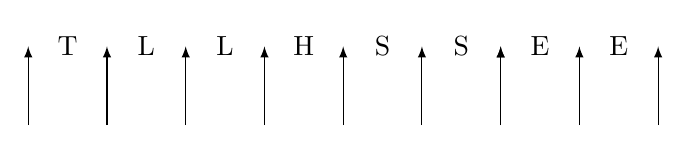
\begin{tikzpicture}
            \node at (0,0) {T};
            \node at (1,0) {L};
            \node at (2,0) {L};
            \node at (3,0) {H};
            \node at (4,0) {S};
            \node at (5,0) {S};
            \node at (6,0) {E};
            \node at (7,0) {E};

            \draw[-latex] (-0.5,-1) -- (-0.5,0);
            \draw[-latex] (0.5,-1) -- (0.5,0);
            \draw[-latex] (1.5,-1) -- (1.5,0);
            \draw[-latex] (2.5,-1) -- (2.5,0);
            \draw[-latex] (3.5,-1) -- (3.5,0);
            \draw[-latex] (4.5,-1) -- (4.5,0);
            \draw[-latex] (5.5,-1) -- (5.5,0);
            \draw[-latex] (5.5,-1) -- (5.5,0);
            \draw[-latex] (6.5,-1) -- (6.5,0);
            \draw[-latex] (7.5,-1) -- (7.5,0);
        \end{tikzpicture}
    \end{center}
    Vemos que hay 9 lugares para ubicar las letras A. Por lo tanto, cuando no tomamos en cuenta las letras A, existen
    $$\frac{8!}{2!2!2!1!1!} = 5 \, 040$$
    formas de arreglar las letras restantes. Tres de estas posiciones se pueden elegir de
    $$\binom{9}{3} = 84 \text{ formas.}$$
    Por la regla del producto existen $5040 \times 84 = 423 \, 360$ disposiciones de las letras de TALLAHASSEE sin letras A consecutivas.
\end{myexample}

\begin{myexample}
    Mostremos que
    $$\binom{n}{r} = \binom{n}{n-r}.$$
    Es fácil (por el principio de esta sección) ver que
    \begin{align*}
        \frac{n!}{r!(n-r)!} & = \frac{n!}{(n-r)!\big(n-(n-r)\big)!} \\
        & = \frac{n!}{r!(n-r)!}.
    \end{align*}
    Por tanto, queda demostrado que
    $$\binom{n}{r} = \binom{n}{n-r}.$$
\end{myexample}

\begin{myexample}
    Para el conjunto 1, 2, 3, 4, 5 mostremos el número de selecciones de tamaño $r = 2$ y de tamaño $n - r = 5 - 2 = 3$ como sigue:
    $$\binom{5}{2} = \frac{5!}{2!(5-2)!} = 10 = \frac{5!}{3!(5-3)!} = \binom{5}{3}.$$
\end{myexample}

\newpage

\begin{theorem}{Teorema del binomio}{}
    Si $x$ e $y$ son variables y $n$ es un entero positivo, entonces
    $$(x + y)^n = \binom{n}{0}x^0y^n + \binom{n}{1}x^1y^{n-1} + \binom{n}{2}x^2y^{n-2} + \cdots + \binom{n}{n-1}x^{n-1}y^1 + \binom{n}{n}x^ny^0.$$
    Utilizando la notación suma
    $$(x + y)^n = \sum_{k=0}^{n} \binom{n}{k} x^ky^{n-k}.$$
    También se puede expresar así:
    $$(x + y)^n = \sum_{k=0}^{n} \binom{n}{n-k} x^ky^{n-k}.$$
    Se pueden intercambiar $x$ e $y$:
    \begin{align*}
        (x + y)^n & = \sum_{k=0}^{n} \binom{n}{k} x^{n-k}y^k \\
        & = \sum_{k=0}^{n} \binom{n}{n-k} x^ny^{n-k}.
    \end{align*}
\end{theorem}

\begin{myexample}
    \begin{enumerate}[label=\alph*)]
        \item Si $n = 3$, entonces:
        \begin{align*}
            (x + y)^3 & = \sum_{k = 0}^{3} \binom{3}{k}x^ky^{3-k} \\
            & = \binom{3}{0}x^0y^{3-0} + \binom{3}{1}x^1y^{3-1} + \binom{3}{2}x^2y^{3-2} + \binom{3}{3}x^3y^{3-3} \\
            & = y^3 + 3xy^2 + 3x^2y + x^3.
        \end{align*}
        También
        \begin{align*}
            (x + y)^3 & = \sum_{j = 0}^{3} \binom{3}{j}x^{3-j}y^j \\
            & = \binom{3}{0}x^{3-0}y^0 + \binom{3}{1}x^{3-1}y^1 + \binom{3}{2}x^{3-2}y^2 + \binom{3}{3}x^{3-3}y^3 \\
            & = x^3 + 3x^2y + 3xy^2 + y^3.
        \end{align*}
        \item Si $n = 4$, entonces:
        \begin{align*}
            (x + y)^4 & = \sum_{r=0}^{4} \binom{4}{r} x^{4-r}y^r \\
            & = \binom{4}{0}x^{4-0}y^0 + \binom{4}{1}x^{4-1}y^1 + \binom{4}{2}x^{4-2}y^2 + \binom{4}{3}x^{4-3}y^3 + \binom{4}{4}x^{4-4}y^4 \\
            & = x^4 + 4x^3y + 6x^2y^2 + 4xy^3 + y^4.
        \end{align*}
    \end{enumerate}
\end{myexample}

\newpage

\begin{corollary}
    \label{SIISNKISUSJD}
    Para cualquier entero $n > 0$,
    \begin{enumerate}[label=\alph*)]
        \item Si $x = 1 = y$, entonces
        $$2^n = \sum_{r=0}^{n} \binom{n}{r}.$$
        \item Si $x = -1$ e $y = 1$, entonces
        $$0 = \sum_{r=0}^{n} \binom{n}{r} (-1)^{n}.$$
    \end{enumerate}
\end{corollary}

\begin{theorem}{Teorema multinomial}{}
    Sean $n$, $t$ enteros positivos. El coeficiente de
    $$x_1^{n_1}, \, x_2^{n_2}, \, x_3^{n_3}, \, \dots, \, x_t^{n_t}$$
    en el desarrollo de
    $$(x_1 + x_2 + x_3 + \cdots x_t)^n$$
    es
    $$\frac{n!}{n_1!n_2!n_3! \cdots n_t!}$$
    donde
    $$n_1 + n_2 + n_3 + \cdots + n_t = n.$$
\end{theorem}

\begin{myexample}
    En el desarrollo de $(x_1 + x_2 + x_3)^4$, tenemos
    \begin{align*}
        (x_1 + x_2 + x_3)^4 & = x_1^4 + 4x_1^3(x_2 + x_3) + 6x_1^2(x_2+x_3)^2 + 4x_1(x_2+x_3)^3 + (x_2+x_3)^4 \\
        & = x_1^4 + 4x_2x_1^3 + 4x_3x_1^3 + 6x_2^2x_1^2 + 6x_3^2x_1^2 + 12x_2x_3x_1^2 + 4x_2^3x_1 \\
        & \hspace{1cm} +4x_3^3x_1 + 12x_2x_3^2x_1 + 12x_2^2x_3x_1 + x_2^4 + x_3^4 + 4x_2x_2^3 + 6x_2^2x_3^2 + 4x_2^3x_3
    \end{align*}
    El coeficiente de $x_1^2x_2^1x_3^1$ en el desarrollo de $(x_1 + x_2 + x_3)^4$ con $n = 4$, $n_1 = 2$, $n_2 = 1$, $n_3 = 1$ es
    $$\frac{4!}{2!1!1!} = 12.$$
    El coeficiente de $x_1^2x_2^0x_3^2$ en el desarrollo de $(x_1 + x_2 + x_3)^4$ con $n = 4$, $n_1 = 2$, $n_2 = 0$, $n_3 = 2$ es
    $$\frac{4!}{2!0!2!} = 6.$$
    El coeficiente de $x_1^0x_2^1x_3^3$ en el desarrollo de $(x_1 + x_2 + x_3)^4$ con $n = 4$, $n_1 = 0$, $n_2 = 1$, $n_3 = 3$ es
    $$\frac{4!}{0!1!3!} =4.$$
    El coeficiente de $x_1^4x_2^0x_3^0$ en el desarrollo de $(x_1 + x_2 + x_3)^4$ con $n = 4$, $n_1 = 4$, $n_2 = 0$, $n_3 = 0$ es
    $$\frac{4!}{4!0!0!} = 1.$$
\end{myexample}

\newpage

\section{Combinaciones con repetición: Distribuciones}

\begin{myexample}
    Siete estudiantes van a un restaurante en donde cada alumno puede seleccionar solo uno de los siguientes platillos:
    \begin{center}
        \begin{tabular}{llcccc}
            Platillo & & Hamburguesa & Pozole & Barbacoa & Ensalada \\
            Letra asignada & & H & P & B & E
        \end{tabular}
    \end{center}
    Una selección posible es
    \begin{center}
        \begin{tabular}{llccccccc}
            Número de estos & & 1 & 2 & 3 & 4 & 5 & 6 & 7 \\
            Selección & & H & H & P & B & E & E & E
        \end{tabular}
    \end{center}
    La selección se puede representar con dos símbolos: $\mid$, $X$
    \begin{center}
        \begin{tabular}{cl}
            $\mid$ & para seleccionar \\
            $X$ & para elegir un platillo
        \end{tabular}
    \end{center}
    donde tenemos las siguientes condiciones:
    \begin{itemize}
        \item Si $X$ está a la izquierda de $\mid$ es: H.
        \item Si $X$ está entre la primer y segunda $\mid$ es: P.
        \item Si $X$ está entre la segunda y tercer $\mid$ es: B.
        \item Si $X$ está a la derecha de la tercer $\mid$ es: E.
    \end{itemize}
    Un ejemplo es:
    \begin{center}
        \begin{NiceTabular}[columns-width=3cm,hvlines-except-borders,rules={color=white,width=1pt}]{cc}
        \CodeBefore
        \rowcolor{jblueleft!80}{1}
        \rowcolors{2}{DodgerBlue3!40}{jblueinner}
        \Body
        \RowStyle[color=white]{}
            Selección & Representación \\
            HHPBEEE & $XX \mid X \mid X \mid XXX$ \\
            HHHPPPE & $XXX \mid XXX \mid \mid X$ \\
            PPBBBEE & $\mid XX \mid XXX \mid XX$ \\
            EEEEEEE & $\mid \mid \mid XXXXXXX$ \\
            PPBBBBE & $\mid XX \mid XXXX \mid X$ \\
            HPPBBBB & $X \mid XX \mid XXXX$ \\
            BBBBBBB & $\mid \mid XXXXXXX \mid$
        \end{NiceTabular}
    \end{center}
    Deducimos que el número de selecciones con repetición es igual con el número de permutaciones con objetos repetidos, en este caso:
    \begin{align*}
        \frac{n!}{n_1!n_2!} & = \frac{10!}{7!3!} \\
        & = \frac{10!}{7!(10-7)!} \\
        & = \binom{10}{7} \\
        & = \binom{10}{3}.
    \end{align*}
\end{myexample}

\newpage

\begin{BOX}
    En general, cuando queremos elegir, con repetición, $r$ de $n$ objetos distintos, vemos que estamos considerando todas las disposiciones de $r$ letras $X$ y $n - 1$ $\mid$, y que su número es
    $$\frac{(n+r-1)!}{r!(n-1)!} = \binom{n+r-1}{r}.$$
    En consecuencia, el número de combinaciones de $n$ objetos tomados de $r$ en $r$, con repeticiones, es $C(n + r - 1, \, r)$.
\end{BOX}

\begin{myexample}
    Una cervecería ofrece 20 tipos de cerveza en lata. Si suponemos que al menos hay una docena de cada tipo cuando entramos a la tienda, podemos elegir una docena de cerveza en lata de
    \begin{align*}
        C(n + r - 1, \, r) & = C(20 + 12 - 1, \, 12) \\
        & = C(31, \, 12) \\
        & = 141 \, 120 \, 525 \text{ formas.}
    \end{align*}
    Notemos que $n = 20$ y $r = 12$.
\end{myexample}

\begin{myexample}
    Un gerente trabaja con cuatro supervisores:
    \begin{center}
        \begin{tabular}{cccc}
            1) Sánchez & 2) Hernández & 3) Gutierrez & 4) López
        \end{tabular}
    \end{center}
    Se van a repartir 100€ entre ellos como incentivo.
    \begin{enumerate}[label=\alph*)]
        \item Si se admite el caso en que una o más de las vicepresidentas no obtenga nada, el gerente hace una selección de tamaño 10 (uno por cada unidad de 10€) de una colección de tamaño 4 (cuatro supervisores), con repetición. Esto puede hacerse de
        \begin{align*}
            C(n + r - 1, \, r) & = C(4 + 10 - 1, \, 10) \\
            & = C(13, \, 10) \\
            & = 286 \text{ formas.}
        \end{align*}
        Mostremos dos de ellas
        \begin{center}
            \begin{tabular}{ccccccccc}
                1 & 1 & 2 & 3 & 3 & 3 & 3 & 3 & 4 \\
                2 & 2 & 2 & 3 & 3 & 3 & 4 & 4 & 4
            \end{tabular}
        \end{center}
        \item Si cada supervisor debe recibir al menos 10€ como mínimo, entonces con esta restricción, el gerente debe hacer ahora una selección de tamaño 6 (los seis billetes restantes) de la misma colección de tamaño 4, y las opciones son ahora
        \begin{align*}
            C(n + r - 1, \, r) & = C(4 + 6 - 1, \, 6) \\
            & = C(9, \, 6) \\
            & = 84.
        \end{align*}
        Por ejemplo, si tenemos $\begin{array}{cccccc}
            2 & 3 & 3 & 4 & 4 & 4
        \end{array}$\!\!, entonces Sánchez recibiría 10€, Hernández recibiría 20€, Gutierrez recibiría 30€ y López recibiría 40€; lo que en total suma 100€.
    \end{enumerate}
\end{myexample}

\newpage

\begin{myexample}
    Un mensaje está formado por 12 símbolos diferentes y se va a transmitir a través de un canal de comunicación. Además de los 12 símbolos, el transmisor también enviará un total de 45 espacios en blanco entre los símbolos, usando al menos tres espacios entre cada par de símbolos consecutivos. ¿De cuántas formas puede el transmisor enviar ese mensaje?

    \tcblower
    \textbf{\color{jblueleft}Solución:} Si asignamos a cada símbolo una letra y a cada flecha los 3 espacios, tenemos:
    \begin{center}
        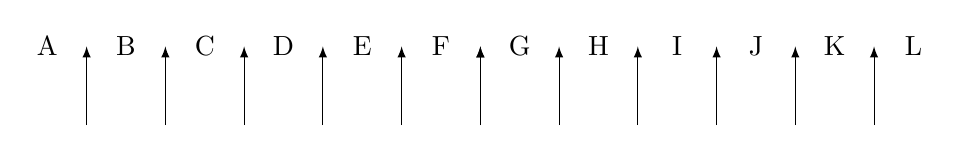
\begin{tikzpicture}
            \node at (0,0) {A};
            \node at (1,0) {B};
            \node at (2,0) {C};
            \node at (3,0) {D};
            \node at (4,0) {E};
            \node at (5,0) {F};
            \node at (6,0) {G};
            \node at (7,0) {H};
            \node at (8,0) {I};
            \node at (9,0) {J};
            \node at (10,0) {K};
            \node at (11,0) {L};
            
            \draw[-latex] (0.5,-1) -- (0.5,0);
            \draw[-latex] (1.5,-1) -- (1.5,0);
            \draw[-latex] (2.5,-1) -- (2.5,0);
            \draw[-latex] (3.5,-1) -- (3.5,0);
            \draw[-latex] (4.5,-1) -- (4.5,0);
            \draw[-latex] (5.5,-1) -- (5.5,0);
            \draw[-latex] (5.5,-1) -- (5.5,0);
            \draw[-latex] (6.5,-1) -- (6.5,0);
            \draw[-latex] (7.5,-1) -- (7.5,0);
            \draw[-latex] (8.5,-1) -- (8.5,0);
            \draw[-latex] (9.5,-1) -- (9.5,0);
            \draw[-latex] (10.5,-1) -- (10.5,0);
        \end{tikzpicture}
    \end{center}
    Hay $12!$ formas de colocar los 12 símbolos diferentes y para cualquiera de estas disposiciones hay 11 posiciones entre los 12 símbolos. Debido a que debe haber al menos tres espacios entre los símbolos consecutivos, utilizamos hasta 33 de los 45 espacios y distribuimos los 12 espacios restantes, pues
    $$- \begin{array}{rl}
        45 & \text{espacios en blanco} \\
        33 & \text{espacios en blanco} \\
        \hline
        12 & \text{espacios en blanco}
    \end{array}$$
    Entonces es una selección con repetición, de tamaño 12 (los espacios) de una colección de tamaño 11 (las posiciones), y puede realizarse de
    \begin{align*}
        C(n + r - 1, \, r) & = C(11 + 12 - 1, \, 12) \\
        & = C(22, \, 12) = 646 \, 646 \text{ formas.}
    \end{align*}
    En consecuencia, por la regia del producto, el transmisor puede enviar tales mensajes con el espacio necesario de
    $$12! \times C(22, \, 12) = 309 \, 744 \, 468 \, 633 \, 600 \text{ formas.}$$
\end{myexample}

\begin{myexample}
    Determine todas las soluciones enteras de la ecuación
    $$x_1 + x_2 + x_3 + x_4 = 7, \quad \text{donde } x_i \geq 0, \quad \text{para toda } 1 \leq i \leq 4.$$

    \tcblower
    \textbf{\color{jblueleft}Solución:} Si tomamos a $x_i$ como el número de monedas entregadas al $i$-ésimo niño, entonces tenemos $n = 4$ que son los niños y $r = 7$ que son las monedas. Así pues, obtenemos
    \begin{align*}
        C(n + r - 1, \, r) & = C(4 + 7 - 1, \, 7) \\
        & = C(10, \, 7) = 120.
    \end{align*}
\end{myexample}

\begin{BOX}
    Los siguientes enunciados son equivalentes:
    \begin{enumerate}[label=\alph*)]
        \item El número de soluciones enteras de la ecuación
        $$x_1 + x_2 + \cdots + x_n = r, \quad \text{donde } x_i \geq 0, \quad \text{para toda } 1 \leq i \leq n.$$
        \item El número  de selecciones, con repetición, de tamaño $r$ de una colección de tamaño $n$.
        \item  El número de formas en que $r$ objetos distintos se pueden distribuir entre $n$ recipientes distintos.
    \end{enumerate}
\end{BOX}

\newpage

\begin{myexample}
    ¿De cuántas formas se puede distribuir 10 canicas rojas (idénticas) en seis recipientes diferentes?

    \tcblower
    \textbf{\color{jblueleft}Solución:} La solución de este problema es equivalente a determinar el número de soluciones enteras no negativas de la ecuación
    $$x_1 + x_2 + x_3 + x_4 + x_5 + x_6 = 10.$$
    Ese número es la cantidad de selecciones de tamaño 10, con repetición, de una colección de tamaño 6. Por lo tanto, la respuesta es
    $$C(6 + 10 - 1, \, 10) = 3 \, 003.$$
\end{myexample}

\begin{myexample}
    ¿Cuántas soluciones enteras no negativas corresponden a la desigualdad
    $$x_1 + x_2 + x_3 + x_4 + x_5 + x_6 < 10?$$

    \tcblower
    \textbf{\color{jblueleft}Solución:} El número de soluciones de la anterior ecuación es equivalente al número de soluciones para la siguiente ecuación:
    $$x_1 + x_2 + x_3 + x_4 + x_5 + x_6 + x_7= 10, \quad \text{donde } x_i \geq 0, \quad \text{para toda } 1 \leq i \leq 6, \quad \text{con } x_7 > 0.$$
    Al sumar $-1$ a ambos lados de la ecuación, obtenemos
    $$x_1 + x_2 + x_3 + x_4 + x_5 + x_6 + \underbrace{x_7 - 1}_{y_{7}} = 10 - 1.$$
    Sean $y_i = x_i$ para $1 \leq i \leq 6$ e $y_7 = x_7 - 1$, así pues, el número de soluciones de la anterior ecuación es el mismo que el número de soluciones enteras no negativas de
    $$y_1 + y_2 + y_3 + y_4 + y_5 + y_6 + y_7= 9, \quad \text{donde } y_i \geq 0, \quad \text{para toda } 1 \leq i \leq 7.$$
    Es decir,
    \begin{align*}
        C(n + r - 1, \, r) & = C(7 + 9 - 1, \, 9) \\
        & = \binom{15}{9} \\
        & = 5 \, 005.
    \end{align*}
\end{myexample}

\begin{myexample}
    En el desarrollo binomial de $(x + y)^r$, cada término es de la forma $\displaystyle \binom{r}{k} x^ky^{r-k}$, con
    $$(x + y)^r = \sum_{k=0}^{r} \binom{r}{k} x^ky^{r-k}.$$
    Por lo que el número total de términos que hay en el desarrollo es el número de soluciones enteras no negativas de 
    $$x_1 + x_2 = r$$
    con $x_1 = k$ y $x_2 = r - k$.
\end{myexample}

\newpage

\begin{myexample}
    Expandiendo el binomio $(x + y)^2$, obtenemos
    \begin{align*}
        (x + y)^2 & = \sum_{k=0}^{2} \binom{2}{k}x^ky^{2-k} \\
        & = \binom{2}{0} x^0y^2 + \binom{2}{1}x^2y^{2-1} + \binom{2}{2} x^2y^{2-2} \\
        & = y^2 + 2xy + x^2.
    \end{align*}
    El número de soluciones de
    $$x_1 + x_2 = 2$$
    con $n = 2$ y $r = 2$ es
    \begin{align*}
        C(n + r - 1, \, r) & = C(2 + 2 - 1, \, 2) \\
        & = C(3, \, 2) \\
        & = 3.
    \end{align*}
    Por tanto, el binomio $(x + y)^2$ tiene 3 términos.
\end{myexample}

\begin{myexample}
    ¿Cuántos términos tiene la expansión
    $$(x + y)^{14} = \sum_{j=0}^{14} \binom{14}{j} x^jy^{14-j}?$$

    \tcblower
    \textbf{\color{jblueleft}Solución:} Sean $x_1 = j$ y $x_2 = 14 - j$. Hallemos el número de soluciones enteras no negativas de
    $$x_1 + x_2 = 14$$
    con $n = 2$ y $r = 14$, obtenemos
    \begin{align*}
        C(n + r - 1, \, r) & = C(2 + 14 - 1, \, 14) \\
        & = C(15, \, 14) \\
        & = 15.
    \end{align*}
    Por tanto, el binomio $(x + y)^{14}$ tiene 15 términos.
\end{myexample}

\begin{myexample}
    Hallemos el número de términos de $(w + x + y + z)^{10}$. Notemos que el número de términos es igual al número de soluciones de la ecuación
    $$y_1 + y_2 + y_3 + y_4 = 10, \quad \text{donde } y_i \geq 0, \quad \text{para toda } 1 \leq i \leq 4.$$
    Procediendo como el anterior ejemplo con $n = 4$ y $r = 10$, obtenemos que $(w + x + y + z)^{10}$ tiene
    \begin{align*}
        C(n + r - 1, \, r) & = C(13, \, 10) \\
        & = 286 \text{ términos.}
    \end{align*}
\end{myexample}